\documentclass[]{article}
\usepackage{tikz}
\usepackage{hyperref}

%opening
\title{CSC373 Stuff Week 8}
\date{}
\begin{document}
\maketitle

\section{Using edges multiple times for flow}
\begin{figure}[h]
	\centering
	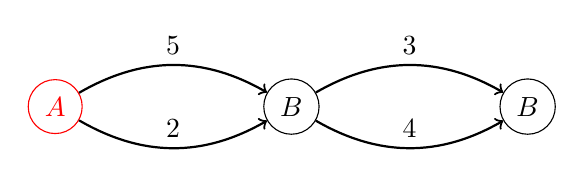
\begin{tikzpicture}
	\node[draw,circle,color=red] (A) at (0,0) {$A$};
	\node[draw,circle] (B) at (3,0) {$B$};
	\node[draw,circle] (C) at (6,0) {$B$};

	
	\draw [->, thick] (A) edge [bend right] node[above] {$2$} (B);
	\draw [->, thick] (A) edge [bend left] node[above] {$5$} (B);
	
	\draw [->, thick] (B) edge [bend right] node[above] {$4$} (C);
	\draw [->, thick] (B) edge [bend left] node[above] {$3$} (C);
	
	\end{tikzpicture}
\\Solve the max flow where the first 2 augmenting paths chosen are (5,3) then (2,4).
\end{figure}


\section{Max Flow with Anti-Parallel Edge}
The following example is from CLRS (26.1).\\
How can we modify this graph to remove all anti-parallel edges such that the max flow does not change? Next, solve the max flow.
%\textit{Encourage the students to read this section. It gives some of the answers for the assignment}
\begin{figure}[h]
	\centering
	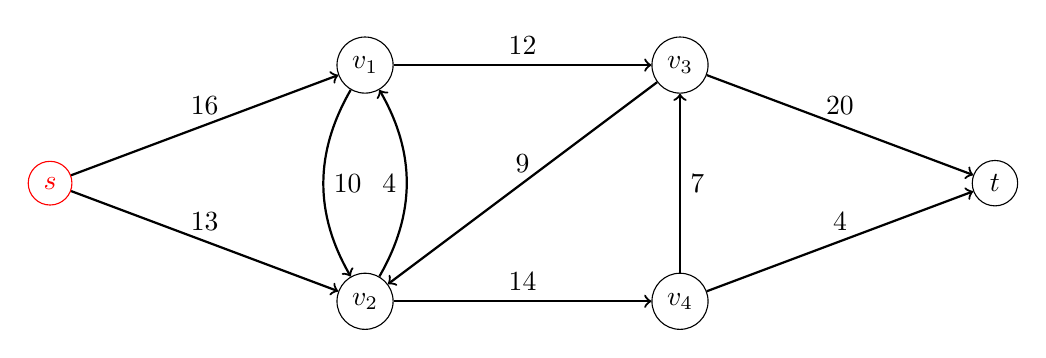
\begin{tikzpicture}
	\node[draw,circle,color=red] (A) at (-4,-1.5) {$s$};
	\node[draw,circle] (C) at (0,0) {$v_1$};
	\node[draw,circle] (D) at (4,0) {$v_3$};
	\node[draw,circle] (F) at (8,-1.5) {$t$};
	
	\node[draw,circle] (B) at (0,-3) {$v_2$};
	\node[draw,circle] (E) at (4,-3) {$v_4$};

	
	\draw [->, thick] (A) edge node[above] {$16$} (C);
	\draw [->, thick] (A) edge node[above] {$13$} (B);
	
	\draw [->, thick] (B) edge node[above] {$14$} (E);
	\draw [->, thick] (B) edge [bend right] node[left] {$4$} (C);
	\draw [->, thick] (C) edge [bend right] node[right] {$10$} (B);
	
	\draw [->, thick] (C) edge node[above] {$12$} (D);
	
	\draw [->, thick] (D) edge node[above] {$20$} (F);
	
	\draw [->, thick] (E) edge node[above] {$4$} (F);
	\draw [->, thick] (E) edge node[right] {$7$} (D);
	
	\draw [->, thick] (D) edge node[above] {$9$} (B);
	
	%\draw [->, thick, color=red] (A) edge node[below] {$1$} (D1);
	%\draw [->, thick, color=red] (A) edge node[below] {$1$} (Dk);
	%\draw [dotted, thick] (D1) edge node[below] {} (Dk);
	
	
	\end{tikzpicture}
\end{figure}

\section{Hospital Rush Max}
Shamama's tutorial covered \href{https://exams-library-utoronto-ca.myaccess.library.utoronto.ca/bitstream/exams/17962/1/csc373h-d16.pdf}{Question 4.b in the 2016 UTM exam.}
%\section{Assignment 3}
%\subsection*{Q4}
%\textit{Review the edge-disjoint max path problem. Help them set up the more general problem where each edge, $e$, can be used at most $k_e$ times and each vertex, $v$, can be used at most $k_v$ times. Draw a diagram and try to get the students to find ways to enforce these constraints. I think that we can help them by explaining the vertex restraint at the end if no one gets it. We just split each vertex into 2, one for the incoming edges and another for the outgoing edges. Connect the pair with an edge with weight $k_v$.}
\end{document}
